% Options for packages loaded elsewhere
\PassOptionsToPackage{unicode}{hyperref}
\PassOptionsToPackage{hyphens}{url}
\documentclass[
  14pt,
]{extarticle}
\usepackage{xcolor}
\usepackage[margin=2cm]{geometry}
\usepackage{amsmath,amssymb}
\setcounter{secnumdepth}{-\maxdimen} % remove section numbering
\usepackage{iftex}
\ifPDFTeX
  \usepackage[T1]{fontenc}
  \usepackage[utf8]{inputenc}
  \usepackage{textcomp} % provide euro and other symbols
\else % if luatex or xetex
  \usepackage{unicode-math} % this also loads fontspec
  \defaultfontfeatures{Scale=MatchLowercase}
  \defaultfontfeatures[\rmfamily]{Ligatures=TeX,Scale=1}
\fi
\usepackage{lmodern}
\ifPDFTeX\else
  % xetex/luatex font selection
\fi
% Use upquote if available, for straight quotes in verbatim environments
\IfFileExists{upquote.sty}{\usepackage{upquote}}{}
\IfFileExists{microtype.sty}{% use microtype if available
  \usepackage[]{microtype}
  \UseMicrotypeSet[protrusion]{basicmath} % disable protrusion for tt fonts
}{}
\makeatletter
\@ifundefined{KOMAClassName}{% if non-KOMA class
  \IfFileExists{parskip.sty}{%
    \usepackage{parskip}
  }{% else
    \setlength{\parindent}{0pt}
    \setlength{\parskip}{6pt plus 2pt minus 1pt}}
}{% if KOMA class
  \KOMAoptions{parskip=half}}
\makeatother
\usepackage{longtable,booktabs,array}
\usepackage{calc} % for calculating minipage widths
% Correct order of tables after \paragraph or \subparagraph
\usepackage{etoolbox}
\makeatletter
\patchcmd\longtable{\par}{\if@noskipsec\mbox{}\fi\par}{}{}
\makeatother
% Allow footnotes in longtable head/foot
\IfFileExists{footnotehyper.sty}{\usepackage{footnotehyper}}{\usepackage{footnote}}
\makesavenoteenv{longtable}
\usepackage{graphicx}
\makeatletter
\newsavebox\pandoc@box
\newcommand*\pandocbounded[1]{% scales image to fit in text height/width
  \sbox\pandoc@box{#1}%
  \Gscale@div\@tempa{\textheight}{\dimexpr\ht\pandoc@box+\dp\pandoc@box\relax}%
  \Gscale@div\@tempb{\linewidth}{\wd\pandoc@box}%
  \ifdim\@tempb\p@<\@tempa\p@\let\@tempa\@tempb\fi% select the smaller of both
  \ifdim\@tempa\p@<\p@\scalebox{\@tempa}{\usebox\pandoc@box}%
  \else\usebox{\pandoc@box}%
  \fi%
}
% Set default figure placement to htbp
\def\fps@figure{htbp}
\makeatother
\setlength{\emergencystretch}{3em} % prevent overfull lines
\providecommand{\tightlist}{%
  \setlength{\itemsep}{0pt}\setlength{\parskip}{0pt}}
\usepackage{multirow}
\usepackage{colortbl}
\usepackage{amssymb}
\definecolor{ganttgreen}{HTML}{6FA84F}
% Cap embedded images at 62% of the text height so figures can share a
% page with text instead of claiming a page alone and leaving big gaps.
\makeatletter
\renewcommand*\pandocbounded[1]{%
  \sbox\pandoc@box{#1}%
  \Gscale@div\@tempa{\dimexpr0.62\textheight\relax}{\dimexpr\ht\pandoc@box+\dp\pandoc@box\relax}%
  \Gscale@div\@tempb{\linewidth}{\wd\pandoc@box}%
  \ifdim\@tempb\p@<\@tempa\p@\let\@tempa\@tempb\fi
  \ifdim\@tempa\p@<\p@\scalebox{\@tempa}{\usebox\pandoc@box}%
  \else\usebox{\pandoc@box}%
  \fi%
}
\makeatother
\usepackage{bookmark}
\IfFileExists{xurl.sty}{\usepackage{xurl}}{} % add URL line breaks if available
\urlstyle{same}
\hypersetup{
  hidelinks,
  pdfcreator={LaTeX via pandoc}}

\author{}
\date{}

\begin{document}

\begin{titlepage}
\centering
\vspace*{0.6cm}
{\LARGE\bfseries PhD MILESTONE 1 REPORT\par}
\vspace{1.5cm}
% --- institutional logo (file lives at docs/diagrams/curtin_logo.png) ---
\IfFileExists{../diagrams/curtin_logo.png}{
\includegraphics[width=7cm]{../diagrams/curtin_logo.png}}{{\large\itshape [\,Curtin logo: save as docs/diagrams/curtin\_logo.png\,]}}\par
\vspace{1.5cm}
{\Large\bfseries Economic Model Predictive Control of a Semi-Autogenous Grinding Mill Circuit: A Modular Energy-Minimising Cost Function 
\par}
\vspace{1.5cm}
{\large\bfseries Batbold Sangi\par}
\vspace{0.25cm}
{\large\bfseries (23897641)\par}
\vfill
{\large\bfseries Faculty of Science and Engineering\par}
\vspace{0.2cm}
{\large\bfseries WA School of Mines: Minerals, Energy and Chemical Engineering\par}
\vspace{0.8cm}
{\small Thesis Chair: Prof George Barakos \\[0.12cm] Principal Supervisor: Prof Agus Saptoro \\[0.12cm] Co-Supervisor: Prof Laurence Dyer \\[0.12cm] Co-Supervisor: Prof Moses Tade \\[0.35cm] August 2026\par}
\vspace{0.3cm}
\end{titlepage}

\tableofcontents
\thispagestyle{empty}
\newpage

\subsection{1. Abstract}\label{abstract}

Semi-autogenous grinding (SAG) is the most energy-intensive stage of
mineral comminution. The comminution circuit dominates a concentrator's
electricity bill and the greenhouse emissions that come with it. The
mill should grind the ore to the size the downstream circuits require,
at the lowest possible energy per tonne, while respecting throughput
demand and product-quality limits. The classical solution places a
steady-state real-time optimiser (SSRTO) above a tracking model
predictive controller (MPC). Ore hardness and feed size drift on
hour-to-shift timescales, so the plant rarely holds the strict steady
state that SSRTO's parameter-estimation step requires. The optimiser
then sits idle and pushes stale set-points. Economic MPC (EMPC) merges
optimisation and regulation into a single receding-horizon problem. It
can track a moving economic optimum during transients, and transients
are where a SAG mill spends most of its operating life.

This research develops and benchmarks an EMPC framework for a SAG
circuit. It uses two prediction models. The Hulbert-Le Roux
reduced-order model handles fast online solves. A cumulative-rates
population balance model (PBM) covers cases that need the full product
size distribution. Two contributions are central. The first is a
modular, energy-minimising cost function. The online controller
minimises mill energy alone. The downstream economics do not enter it
directly. They are worked out offline and reduced to one specification,
a particle-size floor the controller must hold. Re-tuning for a new ore
body or a different downstream plant then means swapping that
specification, not redesigning the controller. The second is a
comparison of the supervisory architectures (SSRTO, ROPA, and single-
and two-layer EMPC) together with the basic regulatory baselines. The
test is not a fixed steady state but a plant-representative,
transient-rich scenario.

Preliminary work has implemented all of these controllers in
\texttt{do-mpc}/CasADi/IPOPT on a simulated eight-state circuit. The
first like-for-like benchmark is now complete. Six 218 h closed-loop
runs compared three architectures (SSRTO over PI loops, single-layer
EMPC and two-layer EMPC) under both economic objectives, on identical
ore, estimator and constraints. Two findings stand out. First, the
specific energy of all six runs clustered within about two percent and
followed the ore hardness. The energy per tonne is set by the ore and
the quality floor, not by the architecture or the objective. Second,
energy minimisation reached the same specific energy as profit
maximisation while keeping the mill away from its feed and speed limits.
This supports the modular mill-level objective the project proposes. The
two-layer EMPC remains the main candidate. These results are synthetic.
The next step is to calibrate the mill model against historical plant
data, so the comparison can carry plant-level numbers.

\newpage

\subsection{Nomenclature}\label{nomenclature}

\textbf{Manipulated variables (MV):} \texttt{MFS} mill feed solids / ore
feed rate (t/h) · \texttt{CFF} cyclone feed flow · \texttt{SFW} sump
feed water · $\phi_c$ mill speed (fraction of critical speed,
0.55-0.80).

\textbf{Controlled variables (CV):} \texttt{JT} total mill charge
filling · \texttt{SVOL} sump slurry volume · \texttt{PSE} product size
estimate (fraction \textless{} 75 µm) · \texttt{Pmill} mill power draw.

\textbf{Plant states (8):} mill \texttt{Xmw,\ Xms,\ Xmf,\ Xmr,\ Xmb}
(water, solids, fines, rocks, balls); sump \texttt{Xsw,\ Xss,\ Xsf}
(water, solids, fines).

\textbf{Disturbances / parameters:} $\alpha_r$ feed rocks fraction ·
$\phi_f$ ore-hardness (power per tonne of fines) · \texttt{MIW} mill
inlet water · \texttt{MFB} ball feed.

\textbf{Derived / economic:} \texttt{TP} throughput ($\approx$ \texttt{MFS} at
steady state) · $\mathrm{SEC}=P_{mill}/\mathrm{MFS}$ specific energy consumption
(kWh/t) · \texttt{A} net return per tonne (\$/t) · \texttt{B}
electricity tariff (\$/kWh) · \texttt{NSR} net smelter return ·
$J_{comm}$ commercial objective.

\textbf{Acronyms:} SAG semi-autogenous grinding · PBM population balance
model · PSD particle-size distribution · (E)MPC (economic) model
predictive control · RTO real-time optimisation · SSRTO steady-state RTO
· ROPA RTO with persistent adaptation · DRTO dynamic RTO · EKF extended
Kalman filter · DO/NDOB (nonlinear) disturbance observer · PINN
physics-informed neural network · OCP optimal control problem · NLP
nonlinear program.

\newpage

\subsection{2. Research Background}\label{research-background}

\subsubsection{2.1 The SAG grinding circuit and its control
problem}\label{the-sag-grinding-circuit-and-its-control-problem}

Comminution is the crushing and grinding of run-of-mine (ROM) ore to
free the valuable mineral. It is the single largest electricity consumer
on a concentrator, and the SAG mill is the largest single draw within
it. The control problem is multivariable and strongly coupled. A closed
circuit (SAG mill → sump → hydrocyclone) is driven through a handful of
manipulated variables: ore feed rate, cyclone feed flow, dilution water
and mill speed. The controller must hold a few controlled variables
(mill charge, sump level, product particle size) inside an operating
envelope. Meanwhile the ore properties drift underneath the controller.
The economically meaningful quantity is the specific energy consumption
(SEC), the energy per tonne of product at acceptable quality. SEC is
also the right variable for comparing controllers, and it is the
headline metric of this project's benchmark. Set-point tracking remains
necessary at the regulatory level. On its own, however, it does not
decide where the plant should operate. Choosing the operating point is
an economic decision.

A controller is only as good as the model behind it, the estimator that
feeds it state, and the supervisory layer that decides \emph{where} to
operate. The next three subsections review each in turn.

\subsubsection{2.2 Control-oriented dynamic
models}\label{control-oriented-dynamic-models}

A control-oriented mill model must be predictive enough to capture the
load, power, and product dynamics. It must also stay cheap enough to
solve inside an online optimisation. Two mechanistic families span this
trade-off, and both are used in this work. A reduced-order lumped model
serves the fast economic MPC. A size-resolved population balance model
serves the cases where the cost function must see the full product size
distribution.

The \textbf{Hulbert-Le Roux reduced-order model} (Le Roux et al., 2013;
Le Roux \& Steyn, 2022) collapses the size structure to three
operationally meaningful lumps: \emph{rocks}, \emph{solids} and
\emph{fines}. Water and ball hold-ups are added, giving a five-state
mill plus a three-state sump in the closed-circuit form. The model's strengths
make it the default for online control. It can be identified from a
single plant survey. It supports non-linear MPC at industrial sample
rates (Coetzee et al., 2010; Le Roux et al., 2016). An EKF state
estimator works well on it, recovering the unmeasured internal states
from standard plant sensors (Le Roux et al., 2017). The model has also
been embedded in an industrial digital twin (Quintanilla et al., 2025).
The model's drawbacks follow from the same lumping, the grouping of
all particle sizes into three bins. The single quality output is
the product particle-size estimate (PSE), the fraction of
cyclone-overflow product passing a specified limit (e.g.~75 µm). The
model therefore represents only one quantile of the size distribution
and never its shape.

The model's core is a set of population volume balances for the mill hold-ups of
water, solids, rocks and fines, in m\textsuperscript{3} (Le Roux et al.,
2013):

\begingroup\small

\begin{equation}\frac{d}{dt}X_{mw}=MIW+V_{cwu}-V_{mwo}\tag{1a}\end{equation}

\begin{equation}\frac{d}{dt}X_{ms}=\frac{MFS}{D_S}\,(1-\alpha_r)+V_{csu}-V_{mso}+RC\tag{1b}\end{equation}

\begin{equation}\frac{d}{dt}X_{mr}=\frac{MFS}{D_S}\,\alpha_r-RC\tag{1c}\end{equation}

\begin{equation}\frac{d}{dt}X_{mf}=\frac{MFS}{D_S}\,\alpha_f+V_{cfu}-V_{mfo}+FP\tag{1d}\end{equation}

\endgroup

Each hold-up gains material from the feed and the cyclone underflow and
loses it through the end-discharge screen (the \(V\) flow terms). A
fifth balance tracks the ball hold-up. The feed ore splits by two ore
parameters. The fraction \(\alpha_r\) enters as rocks, too large to
discharge. The fraction \(\alpha_f\) enters as fines, already below the
specification size. Breakage moves material down this ladder, and in
this model it is driven by mill power:

\begingroup\small

\begin{equation}RC=\frac{P_{mill}\,\varphi}{D_S\,\phi_r}\cdot\frac{X_{mr}}{X_{mr}+X_{ms}}\tag{2a}\end{equation}

\begin{equation}FP=\frac{P_{mill}}{D_S\,\phi_f\left[1+\alpha_{\phi_f}\left(\frac{LOAD}{v_{mill}}-v_{P_{max}}\right)\right]}\tag{2b}\end{equation}

\endgroup

where \(RC\) is the volumetric rate at which rocks are consumed into
solids and \(FP\) the rate at which new fines are produced. The two
ore-hardness parameters sit exactly here. \(\phi_r\) (kWh/t) is the rock
abrasion factor, the energy required per tonne of rocks broken.
\(\phi_f\) (kWh/t) is the power needed per tonne of fines produced, the
ore-hardness parameter used throughout this report. The factor
\(\varphi\) is the slurry rheology factor, and \(\alpha_{\phi_f}\) is a
small correction for the mill filling (\(LOAD\) is the total charge
volume and \(v_{mill}\) the mill volume). Mill power itself is an
empirical parabola in the charge and the rheology, scaled by the mill
speed (Le Roux et al., 2013):

\begingroup\small

\begin{equation}P_{mill}=P_{max}\left\{1-\delta_{Pv}Z_x^{2}-2\chi_P\,\delta_{Pv}\,\delta_{Ps}\,Z_x Z_r-\delta_{Ps}Z_r^{2}\right\}\,(\alpha_{speed})^{\alpha_P}\tag{3}\end{equation}

\endgroup

where \(Z_x\) measures the charge volume against the filling at maximum
power, \(Z_r\) measures the rheology factor against its value at maximum
power, and \(\alpha_{speed}\) is the fraction of critical mill speed
(written \(\phi_c\) elsewhere in this report).

The \textbf{cumulative-rates population balance model} resolves the full
PSD. It tracks the ore mass in each of $n$ geometrically-spaced
size classes, giving a $2n{+}2$-state circuit ($n$ mill
classes plus mill water, $n$ sump classes plus sump water). Its
defining feature is the cumulative-rates parametrisation of Hinde \&
Kalala (2009). A standard PBM describes breakage with two functions that
are hard to measure: a specific breakage-rate function and a
breakage-distribution function. Their parameters are back-calculated
from test data and are notoriously sensitive to measurement error, with
large variances. The cumulative-rates form replaces both with a single
cumulative breakage rate $K_i^{E}$. This is the rate at which
material coarser than size $x_i$ breaks below that size, normalised by
mill power so that the rate is largely insensitive to scale-up. The decisive advantage of the cumulative-rates form is direct
estimation. $K_i^{E}$ comes straight from
measured feed and product size distributions and the mill's specific
energy input, with no back-calculation. That makes a PSD-resolving model
robustly identifiable, and smooth enough to linearise or differentiate
for control.

For size class $i$ the model tracks the mass $w_i$ held
in the mill, with $W_i$ the mass coarser than size $x_i$
(Le Roux \& Craig, 2013):

\begingroup\small

\begin{equation}\frac{dw_i}{dt}=f_i-g_i w_i+W_i\,\frac{P}{M}K_i^{E}-\left(w_i+W_i\right)\frac{P}{M}K_{i+1}^{E}\tag{4}\end{equation}

\endgroup

where $f_i$ is the feed rate into the class, $g_i$ its
discharge rate, $P$ the net mill power and $M$ the ore
hold-up. The first power term is material breaking into the class from
coarser sizes. The second is material breaking out of it to finer sizes.
The energy-normalised rate $K_i^{E}=(M/P)\,K_i$, in
$(\mathrm{kWh/t})^{-1}$, is the scale-robust quantity described above, and it is
where the ore hardness lives in this model. Harder ore means smaller
$K_i^{E}$ values, fewer tonnes broken below each size per kWh
of grinding energy. The whole rate curve is captured by one smooth
fitted function (Le Roux \& Craig, 2013):

\begingroup\small

\begin{equation}\hat{K}_i^{E}=\kappa_1\,\frac{x_i^{\alpha_1}}{1+\left(x_i/\mu\right)^{\lambda}}+\kappa_2\,x_i^{\alpha_2}\tag{5}\end{equation}

\endgroup

with six ore-dependent parameters \(\kappa_1\), \(\kappa_2\),
\(\alpha_1\), \(\alpha_2\), \(\mu\) and \(\lambda\). Together they play
the role that the single \(\phi_f\) plays in the reduced-order model,
spread over the full size axis.

The two families are complementary rather than competing. The Hulbert-Le
Roux model is preferred for online MPC. Its small state keeps the
optimisation cheap and offers the right granularity for
grinding-circuit-only (PSE-based) economic decisions. The
cumulative-rates PBM is needed when the cost function must see PSD
shape, for example when downstream flotation and leaching kinetics are
size-dependent. Any genuinely plant-wide economic objective requires a
PSD-resolving signal that a single PSE quantile cannot provide. The
reduced $n=5$ or $9$ form supplies that at a state count a
controller can still afford.

\subsubsection{2.3 Disturbance observers and state
estimation}\label{disturbance-observers-and-state-estimation}

A SAG circuit's disturbances are well characterised and act on distinct
timescales. Ore-hardness drift acts hour-to-shift and is the dominant
source of model-plant mismatch. Feed-size variability acts on
minutes-to-hours and is usually correlated with hardness. Feed-moisture
and dilution-water swings change the slurry rheology. Liner wear and
ball-charge drift act over weeks to months. The literature splits the
estimation work across two roles. A fast non-linear disturbance observer
(NDOB) at the regulatory MPC layer cancels input-side disturbances by
feed-forward before they reach the optimisation loop. The first
grinding-circuit deployments (Chen et al., 2009; Yang et al., 2010)
established two things. Pairing a DO with the MPC improves disturbance
rejection without changing the controller's normal set-point tracking. The estimate also stays
meaningful to operators, who can read it directly as an ``ore-hardness
offset''. The second role is a slow estimator at the economic layer, an
augmented EKF/UKF (Le Roux et al., 2017). It tracks the drifting
hardness parameter and recovers the unmeasured internal mill states. The augmented
Kalman filter is the established choice for this role on grinding
circuits. It propagates the slow parameter drift through its
process-noise model while staying a deterministic, real-time update.
Here the augmented estimator tracks a single slow parameter, the ore
hardness $\phi_f$ (the power drawn per tonne of fines produced). One
direction this work will explore is augmenting it with further
slowly-varying disturbance states, such as the feed rocks fraction
$\alpha_r$ and other rheology-related parameters. The test is whether
jointly estimating them, rather than $\phi_f$ alone, sharpens the
economic-layer model under the realistic, multi-disturbance scenario.

\subsubsection{2.4 The supervisory-optimisation continuum: SSRTO → ROPA
→ DRTO →
EMPC}\label{the-supervisory-optimisation-continuum-ssrto-ropa-drto-empc}

The question \emph{``how does the controller decide what the
economically best operating point is?''} has four published answers.
\textbf{Classical SSRTO} (Darby et al., 2011) puts a separate
steady-state optimiser above the MPC. It solves a parameter-estimation
and economic optimisation problem whenever a steady-state detector
declares the plant settled. Between detections the set-points are held.
The wait is necessary. Fitting the steady-state model to transient data
corrupts it. For a SAG mill this is a real problem. The plant rarely
holds the strict steady state the detector requires, so the optimiser
sits idle and pushes stale set-points.

\textbf{ROPA} (real-time optimisation with persistent adaptation) breaks
SSRTO's central coupling. It runs a continuous dynamic estimator for the
model parameters, so the still-steady-state economic NLP always receives
fresh parameters, even during transients. \textbf{DRTO} replaces the
static NLP with a dynamic optimisation over a long horizon. It emits an
economic \emph{trajectory} for a tracking MPC to follow. \textbf{EMPC}
(Ellis et al., 2014; Faulwasser \& Pannocchia, 2018) takes the DRTO
logic to its limit. It drops the dedicated upper layer and embeds the
economic objective directly in the regulatory MPC's stage cost. DRTO and
EMPC are theoretically equivalent. They share the same dynamic economic
cost, model and horizon, and differ only in whether the layers are kept
visibly separate. An experimental-rig comparison (Matias et al., 2022)
reports ROPA matching DRTO at about 38 \% profit improvement over a
fixed-input baseline, while SSRTO reaches only about 20 \%. The
practical ordering is EMPC $\approx$ DRTO \textgreater{} ROPA \(\gg\) SSRTO.

\subsubsection{2.5 EMPC on grinding circuits - the empirical
record}\label{empc-on-grinding-circuits---the-empirical-record}

The components have been published piecewise. Thivierge, Bouchard and
Desbiens (2023) provide the closest precedent. They compare four
controllers on a simulated HPGR, ball mill and flotation circuit: basic
regulatory control (BRC), advanced regulatory control (ARC), a profit
EMPC, and a power-penalised EMPC. The economic cost function is
flotation-concentrate revenue minus the energy cost. Three of their
results matter here. The basic regulatory baseline used significantly
more energy than the optimising controllers. The ARC and the profit EMPC
performed identically, because the economic optimum sits at the process
constraints and both end up holding the plant there. The power-penalised
EMPC cut specific energy by only 0.4 to 2.9 percent relative to the
profit optimum, and gave up 3.6 to 3.9 percent of net value for it.
However, they evaluate only at steady-state operating points after the
simulator re-settles, and defer transient performance to future work.
The transient-rich benchmark of this project takes exactly that missing
step, and where the two studies overlap, our first six-run results agree
with theirs. Numbi \& Xia
(2016) demonstrate energy-cost EMPC on a crushing plant under
time-of-use tariffs. Jia et al.~(2020) demonstrate multi-stage EMPC for
downstream gold cyanidation. No single study combines the Hulbert-Le
Roux model, a composite DO + augmented-EKF estimator stack, and an
explicit specific-energy EMPC cost on a SAG circuit, evaluated under
realistic operating conditions.

\subsection{3. Research Gap and Problem
Statement}\label{research-gap-and-problem-statement}

The literature reviewed in Section 2 traces a body of work in which
every component of an EMPC for a SAG circuit has been published. They
have never been assembled into a single closed-loop study. They have
also never been exercised under the conditions an industrial SAG mill
actually experiences. Three connected gaps follow.

\textbf{Gap 1 - Architectural integration on a SAG circuit.} No
published study integrates a regulatory-layer DO, an upper-layer
augmented EKF/UKF, and an economic stage cost into a single closed-loop
SAG-mill controller. The two estimator approaches address complementary
timescales but have evolved independently. DO + MPC cancels fast
input-side disturbances at the regulatory clock. The augmented-KF approach
absorbs slow parameter drift at the economic clock.

\textbf{Gap 2 - Realistic operating conditions in evaluation.}
Industrial SAG mills settle at \emph{operational} steady state often,
but the underlying conditions never do. Ore hardness drifts
hour-to-shift. Liner wear changes the mill geometry over weeks to
months. The plant therefore moves between mildly suboptimal operating
points rather than running at the economic optimum. Published
grinding-circuit studies report performance under tightly controlled
conditions instead: step disturbances at fixed operating points, with
metrics sampled after re-settling. Two things have not been quantified.
The first is how a SAG-mill EMPC behaves under disturbance sequences
that resemble actual plant operation. The second is how large the
economic opportunity is that EMPC could capture by tracking the moving
optimum during transients. This quantification is the prerequisite for
any fair head-to-head comparison of EMPC against SSRTO, ROPA, or DRTO.

\textbf{Gap 3 - Cost-function scope on a SAG circuit.} The plant-wide
framework of Le Roux \& Craig (2019) and the flotation-revenue cost of
Thivierge (2023) both argue that the mill's economic objective should
pull from downstream plant signals. Most grinding-circuit EMPC studies
accordingly adopt a revenue- or profit-based stage cost. Two problems
with that choice on a single-stage SAG mill have gone unaddressed. The
first is a scale mismatch. A profit term such as
$A(\mathrm{PSE})\,\mathrm{TP}-B\,P_{mill}$ prices the product through a per-tonne
return $A(\mathrm{PSE})$. That one number collapses recovery, grade, metal
price and downstream constraints. All of these belong to the plant. The
mill controller cannot measure or control them. Embedding these
downstream economics in the mill controller couples it to a calibrated
flotation model, a specific ore body and a specific market state. The
controller must then be re-identified whenever any of these change. The
second problem is a trivial optimum. Even with $A$ known, revenue
scales with throughput while energy is a small per-tonne penalty.
Maximising the profit form therefore simply drives mill speed
$\phi_c$ and feed \texttt{MFS} to their limits. The mill runs
flat out against its throughput and overload constraints. That is a
maximum mode that needs no optimiser, not a meaningful interior optimum.

A complementary and unexplored direction resolves both problems: lift
the revenue term out of the mill controller entirely. The plant-wide
layer sets the product-size floor and the throughput demand. The mill
controller minimises mill energy for those targets. The stage cost is
composed from a small, extensible library of mill-owned terms. The
library holds mill energy ($B\,P_{mill}$), specific energy consumption
(SEC, energy per tonne of feed ore), and penalties on mill-specific
quantities such as residence time. With a size-resolved PBM it can also
penalise the coarse tail of the product PSD. Terms are used singly or in
combination, and weighted, as the downstream specification requires.

The two levels meet at a two-number interface. The first number is the
throughput demand, a floor on \texttt{MFS}. The plant-wide
optimisation, which sees all circuits, decides it and hands it down. The
second is the product-size floor, set by the downstream circuits'
requirements. Inside those limits the mill runs autonomously and never
needs to maximise \texttt{MFS} itself. Re-targeting the mill is a
change of two numbers rather than a re-identification. Neither the
modular framing nor any of these mill-local objectives has yet been
instantiated as the closed-loop cost function of a single-stage SAG
mill.

These three gaps define the problem this thesis addresses: to build an
integrated single-stage SAG-mill EMPC with a composite DO +
augmented-estimator stack, to give it a modular energy-minimising cost
function, and to benchmark it honestly against the full RTO/EMPC
architecture spectrum under operating conditions representative of a
real plant.

\begin{center}\rule{0.5\linewidth}{0.5pt}\end{center}

\subsection{4. Aims and Objectives}\label{aims-and-objectives}

The aim of this research is to develop and rigorously evaluate an
economic model predictive control framework for a single-stage SAG
grinding circuit that minimises specific energy consumption under
realistic operating conditions, and to establish where it offers a
genuine advantage over the established real-time-optimisation
architectures. This aim is pursued through four objectives.

\begin{enumerate}
\def\labelenumi{\arabic{enumi}.}
\item
  \textbf{Implement and validate the integrated control stack.} Build
  the single-stage SAG controller in \texttt{do-mpc}/CasADi/IPOPT and
  verify closed-loop regulation against the simulated plant. The
  controller runs on both the Hulbert-Le Roux reduced-order model and
  the cumulative-rates PBM, used in parallel according to the strengths
  and drawbacks of each (Section 2.2). Estimation uses the EKF /
  augmented EKF plus a fast disturbance observer. \emph{(Substantially
  complete.)}
\item
  \textbf{Formulate a modular, energy-minimising EMPC cost function.}
  Derive and implement a stage cost in which the downstream plant
  economics enter only through an offline-derived particle-size
  specification (a one-sided PSE/PSD floor). The online controller then
  minimises mill energy at the demanded throughput and quality.
  Demonstrate the modularity claim: adapting to a new ore body or
  downstream topology is a swap of the specification interface, not a
  controller redesign (the interface is detailed in Section 6.2).
  Explore modular cost functions suited to both single- and multi-stage
  SAG circuits, where each mill's local objective couples to the next
  only through the specification interface. \emph{(Primary
  contribution.)}
\item
  \textbf{Construct a realistic transient scenario and benchmark the
  architectures.} Build a plant-representative, transient-rich operating
  scenario calibrated to historical plant data. It combines ore-hardness
  drift, feed-size variability, and operating-point changes that drive
  the plant between steady states. Use it to compare SSRTO, ROPA, and
  single- and two-layer EMPC against a decentralised-PI / tracking-MPC
  baseline, on specific energy consumption and constraint compliance.
  \emph{(Primary contribution.)}
\item
  \textbf{Develop a PINN surrogate for online tractability.} Train a
  physics-informed neural-network surrogate offline on PBM-simulated
  data. Substitute it for the mechanistic prediction model inside the
  EMPC. The goal is to keep the online optimisation tractable as model
  fidelity and horizon length grow.
\end{enumerate}

\textbf{Scope and priority.} Objectives 1-3 form the core of the
candidature and are largely instantiated in the preliminary work.
\textbf{Objectives 2 and 3 are the central novel contributions} (the
modular cost function and the transient benchmark). Objective 4 (PINN)
is optional. It is pursued only if online solves become too slow as the
horizon and model detail grow. Otherwise the mechanistic model stays the
default. This staging keeps the thesis deliverable even if Objective 4
yields negative or partial results.

\begin{center}\rule{0.5\linewidth}{0.5pt}\end{center}

\subsection{5. Significance and Novelty}\label{significance-and-novelty}

\subsubsection{5.1 Theoretical
contributions}\label{theoretical-contributions}

This work would be the first to bring three pieces together inside a
single closed-loop SAG-mill controller: a regulatory-layer disturbance
observer, an upper-layer augmented EKF, and an explicit specific-energy
economic stage cost. That closes the architectural gap the component
literature leaves open (Gap 1). The modular spec-interface cost function
(Objective 2) is a novel framing of the plant-wide economic objective.
It separates the offline downstream-economics question from the online
control problem. The transient-scenario benchmark (Objective 3) provides
the first quantification on a SAG mill of the economic opportunity EMPC
captures during transients. That measurement is what any honest
EMPC-vs-RTO comparison requires.

\subsubsection{5.2 Practical
contributions}\label{practical-contributions}

The outcome is a portable, energy-minimising SAG-mill controller. Its
economic objective can be retargeted to a different ore body or
concentrator configuration by replacing an offline-derived
specification, not by re-engineering the controller. That lowers the
barrier to industrial reuse. The transient-scenario study yields
credible, plant-representative specific-energy-saving figures rather
than figures from a benign synthetic test. Practitioners gain a
defensible basis for deciding between an RTO retrofit and a full EMPC.

EMPC has clear advantages over classical RTO, yet it is rarely used in
operating plants. Two practical barriers explain much of the gap. The
first is the well-documented bang-bang issue. When the quality floor is
already satisfied, the energy cost is nearly flat in feed. With no clear
optimum, the controller swings between its actuator bounds. The second
barrier is complexity at the plant-wide level. There, economic
calculations at the plant-wide level run together with planning and
scheduling information and with the dynamics of many units, so
steady-state calculations remain the practical choice. This project reduces both barriers. Modularity removes
part of the plant-wide complexity. The plant-wide layer hands the mill
its required interface values for variables such as \texttt{PSE} and
\texttt{TP}, instead of implementing the mill inside its own
optimisation. The two-layer EMPC at the SAG mill reduces the volatile
bang-bang issue significantly using the longer horizon at the upper
layer. It
also separates the economic decision from the moment-to-moment
actuation. Using
complex cost functions, such as a moving average of SEC, has the
potential to remove the volatile swings completely.

Comminution dominates concentrator electricity use. Grinding alone can
draw up to roughly 80 \% of a concentrator's energy. Even
single-digit-percent specific-energy reductions therefore translate into
material cost and emissions savings at industrial scale. By cutting
grinding electricity demand and the associated greenhouse emissions, the
project supports Western Australia's Net Zero by 2050 commitment. It
also aligns with Curtin University's research direction in sustainable
mineral processing.

\subsection{6. Research Methodology}\label{research-methodology}

The methodology is organised in three parts: the process under study and
its control problem (Section 6.1), the control architecture proposed for
it (Section 6.2), and the forward work plan that delivers and evaluates
the contributions phase by phase against the objectives of Section 4
(Section 6.3).

\subsubsection{6.1 The single-stage SAG grinding mill
circuit}\label{the-single-stage-sag-grinding-mill-circuit}

The case study throughout is a single-stage grinding mill circuit closed
by a hydrocyclone (Figure 1). This is the configuration most commonly
used for single-stage grinding and the standard testbed for
grinding-circuit control (le Roux et al., 2013). Its three elements are
a SAG mill, a sump, and a cyclone.

\begin{center}

\pandocbounded{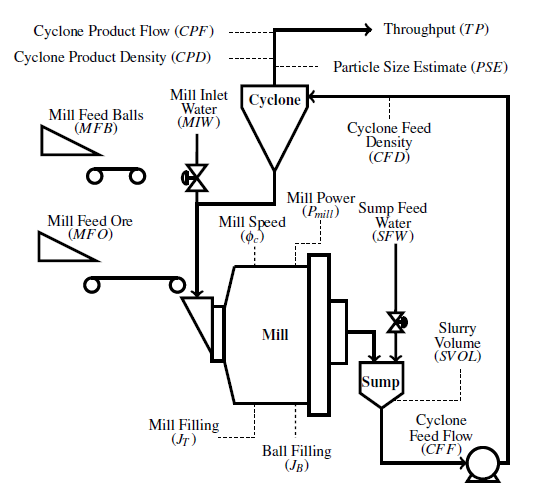
\includegraphics[keepaspectratio]{../diagrams/SAGmill.png}}

\end{center}

{\small \textbf{Figure 1.} The single-stage SAG grinding mill circuit (after le
Roux et al., 2013): SAG mill, sump, and cyclone, with the manipulated
variables (\texttt{MFS}, \texttt{CFF}, \texttt{SFW}, $\phi_c$), the
controlled variables (\texttt{JT}, \texttt{SVOL}, \texttt{PSE},
\texttt{Pmill}), and the circuit outputs (throughput \texttt{TP},
cyclone-feed density \texttt{CFD}, cyclone product flow \texttt{CPF} and
density \texttt{CPD}).\par}

Run-of-mine ore (\texttt{MFS}), steel balls (\texttt{MFB}), and inlet
water (\texttt{MIW}) are fed to the mill. The mill is driven at a
fraction of critical speed ($\phi_c$). It grinds the charge and
discharges slurry to the sump. Dilution water (\texttt{SFW}) sets the
density there, and the cyclone feed pump delivers the slurry at flow
\texttt{CFF} to the cyclone. The cyclone returns coarse underflow to the
mill and sends fine overflow out as product. The manipulated variables
are therefore the ore feed rate \texttt{MFS}, the cyclone feed flow
\texttt{CFF}, the sump dilution water \texttt{SFW}, and the mill speed
$\phi_c$. The controlled variables are the mill charge filling
\texttt{JT}, the sump slurry volume \texttt{SVOL}, and the product
particle-size estimate \texttt{PSE} (the fraction of overflow finer than
a target mesh). Mill power \texttt{Pmill} is monitored as a load and
overload indicator. Throughput \texttt{TP} (the product mass rate,
approximately \texttt{MFS} at steady state) and \texttt{PSE} are the
circuit's economic outputs.


\subsubsection{6.2 Control architecture}\label{control-architecture}

The circuit runs under disturbances on distinct timescales. Ore hardness
($\phi_f$) drifts hour-to-shift and is the dominant source of
model-plant mismatch. Feed size and the feed rocks fraction
($\alpha_r$) vary over minutes to hours. Liner wear and ball-charge
drift act more slowly. The control objective is economic: grind to the
required size at the demanded throughput for the least specific energy,
while holding the mill inside its safe operating envelope.

\begin{figure}[p]
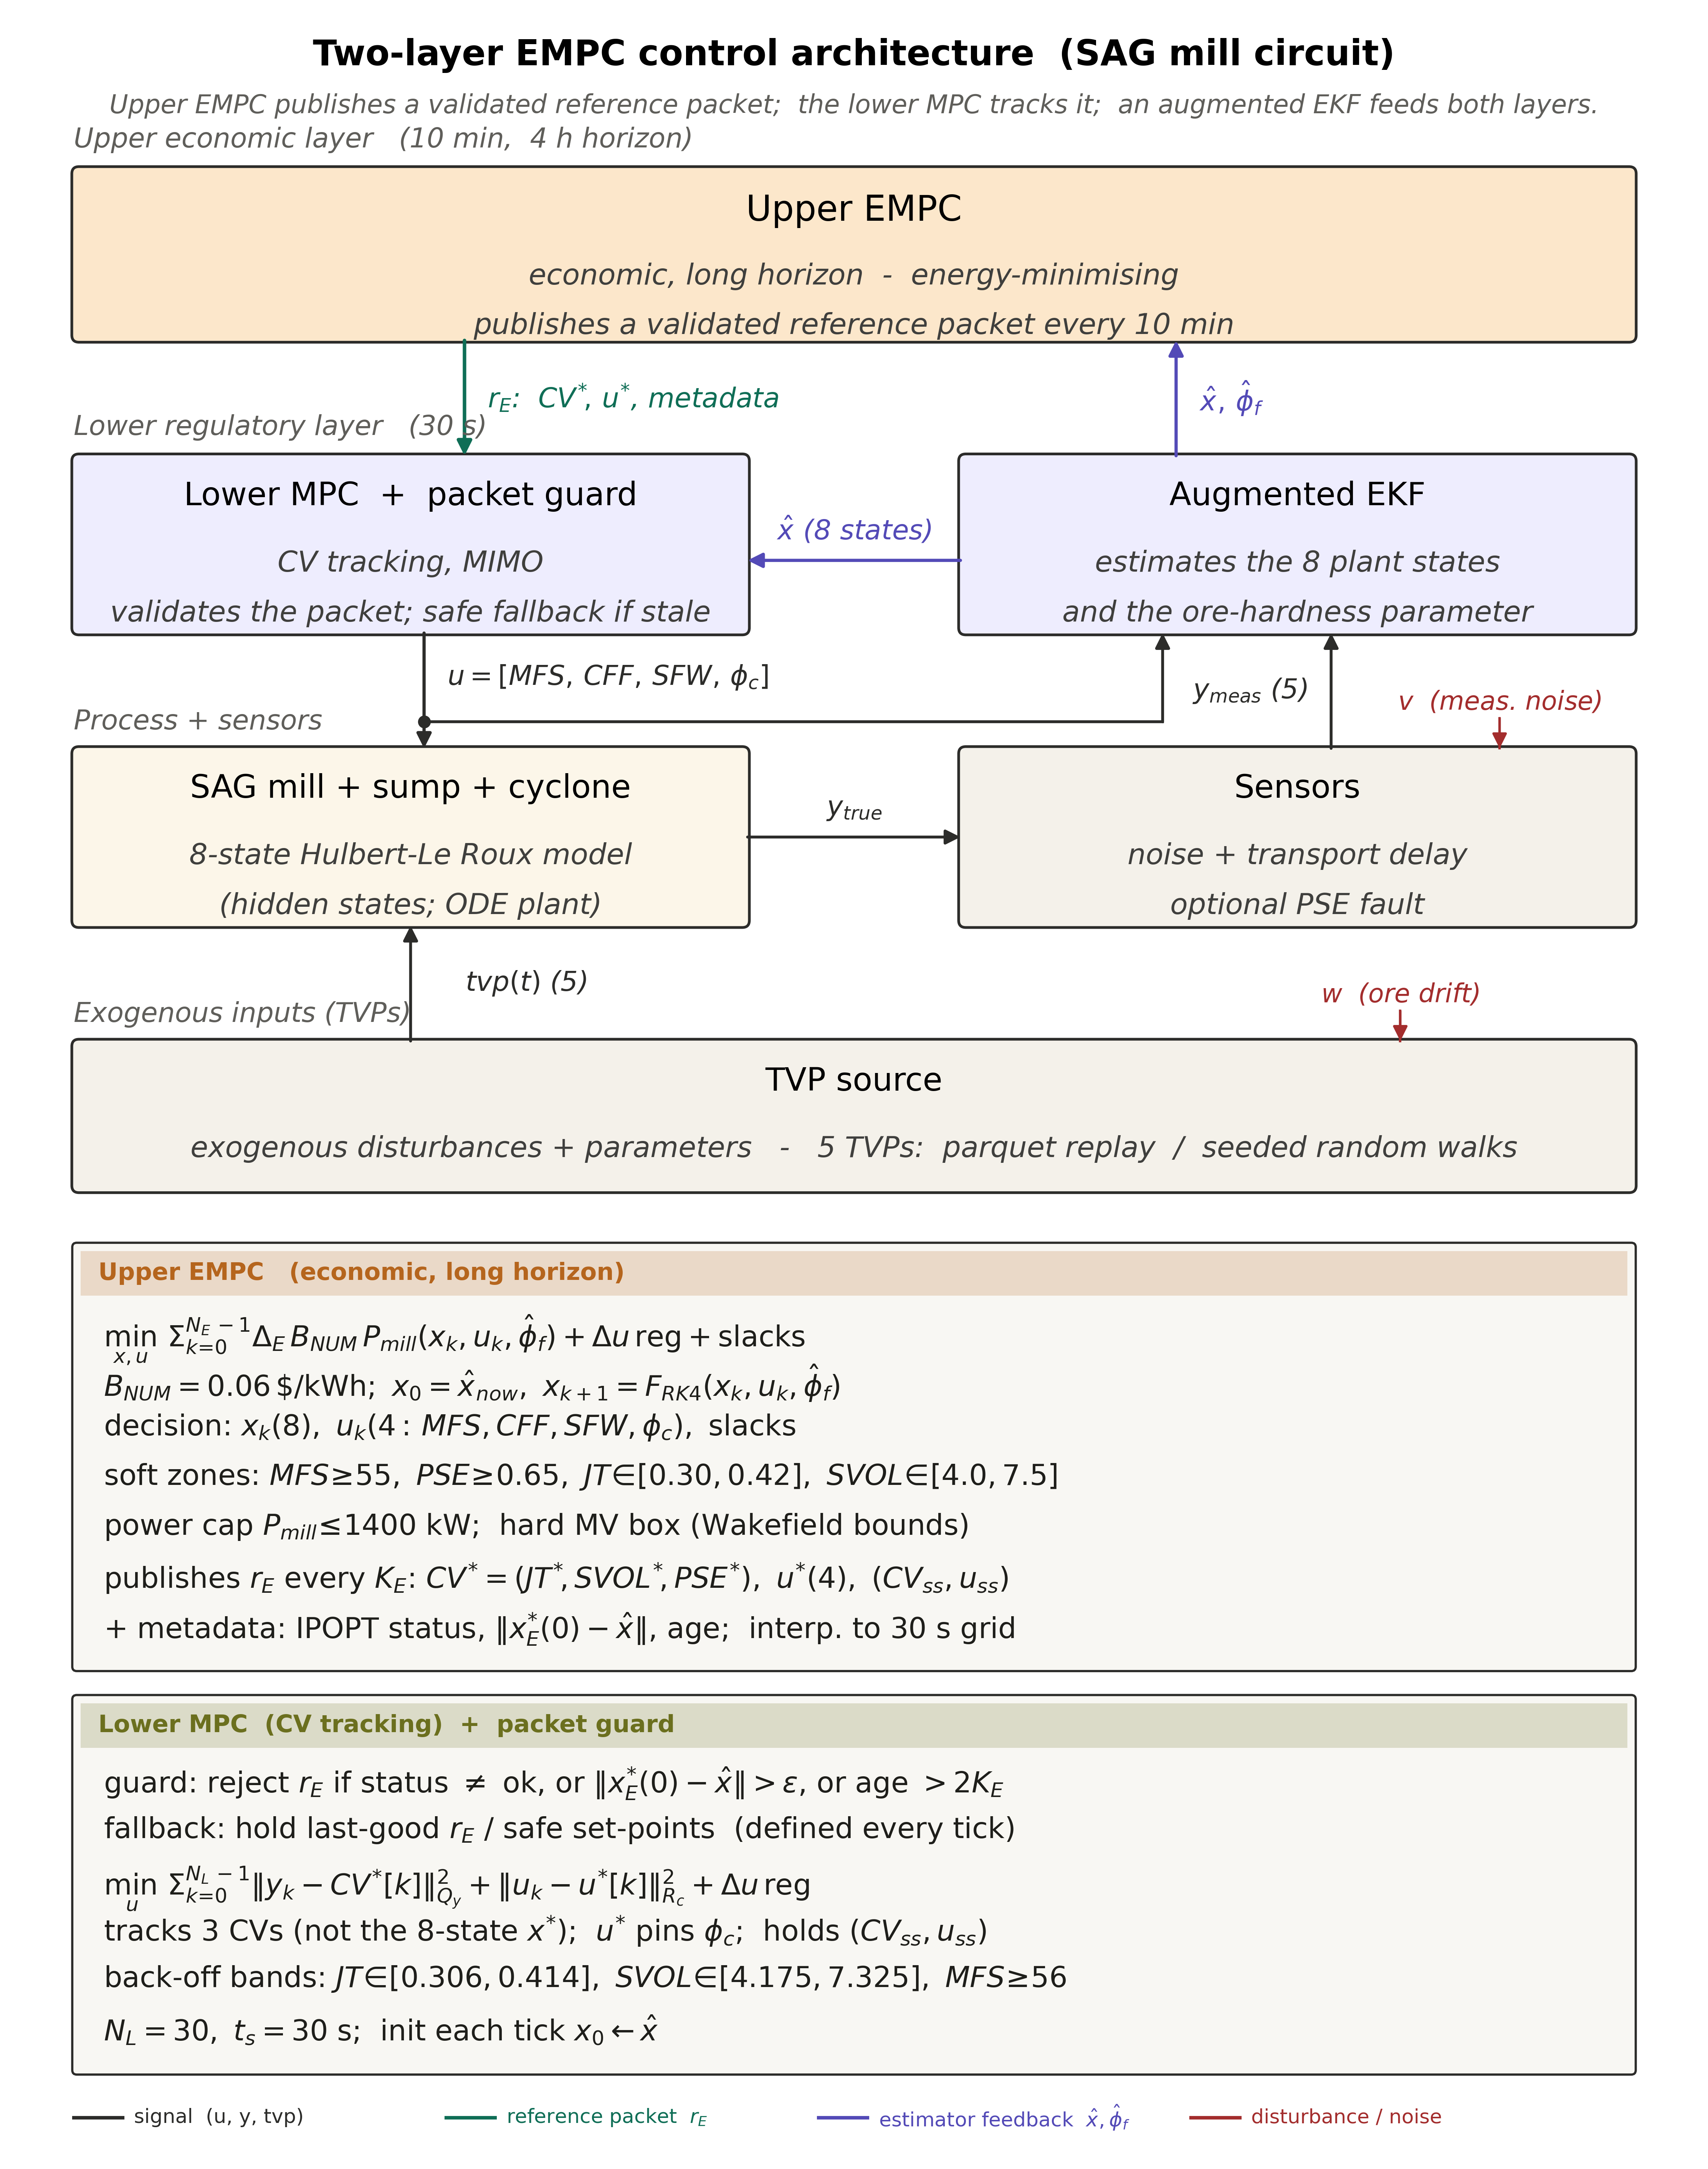
\includegraphics[width=\linewidth,height=0.85\textheight,keepaspectratio]{../diagrams/empc_2layer_v2_milling_circuit.png}

{\small \textbf{Figure 2.} The two-layer EMPC control architecture: the upper
EMPC (economic, long horizon) publishes a validated reference packet
(\texttt{CV*}, \texttt{u*}) through a packet guard to the lower
CV-tracking MIMO MPC; an augmented EKF estimates the mill and sump
states plus the ore-hardness parameter, and a disturbance/parameter
(TVP) source drives the simulated plant.\par}
\end{figure}

Figure 2 shows the
two-layer EMPC realisation. At the regulatory clock, a fast non-linear
disturbance observer cancels input-side disturbances and a lower MIMO
MPC tracks references. At the economic clock, an upper EMPC computes the
economically-optimal operating policy over a long horizon, with all four
MVs as decision variables. The upper layer does not drive the plant
directly. It publishes a reference packet, the CV and MV trajectories
\texttt{CV*} and \texttt{u*}. A packet guard validates each packet on
solver status, initial-state residual, and age before the lower MPC
tracks it. When a solve is rejected, the guard falls back to the last
valid packet or a safe set-point. An augmented extended Kalman filter
estimates the eight mill and sump states together with the slow
ore-hardness parameter $\phi_f$, and feeds both layers.

The economic objective enters the upper EMPC as the modular, mill-local
stage cost of Objective 2. The online cost minimises a composable
mill-owned term (mill energy, specific energy consumption, or another
term from the library of Section 3) subject to the offline-derived
particle-size floor. The prediction step uses the two model families of
Section 2.2, the Hulbert-Le Roux model for fast online solves and the
cumulative-rates PBM where the cost must resolve the product size
distribution.

\subsubsection{6.3 Forward work plan}\label{forward-work-plan}

The remaining programme is organised into four phases mapped to the
objectives of Section 4. Each phase states its method and deliverable.

\textbf{Phase A - Mill-model calibration and transient-scenario
construction (Objectives 1 and 3).} \emph{Method.} Obtain historical
operating data for a SAG circuit under a data-sharing agreement (Section
8). Fit the Hulbert-Le Roux and cumulative-rates parameters to it.
Distinguish identifiable parameters from the historical data, and
validate against held-out operating periods. From the same data,
construct a plant-representative input sequence. The sequence combines
ore-hardness drift and feed variability, calibrated in amplitude and
timescale. It adds operating-point changes that drive the plant between
steady states. These transitions are where the supervisory
architectures are expected to separate. Characterise the sequence by
the fraction of runtime spent in transient
versus operational steady state.

\emph{Deliverable.} A plant-calibrated
mill model with a documented identifiability analysis, together with a
reproducible transient scenario and its documented statistics.

\textbf{Phase B - Modular energy-minimising cost-function formulation
(Objective 2).} \emph{Method.} Formalise the specification interface.
Compile the downstream economics offline into a per-tonne return
\texttt{A} and a one-sided PSE/PSD floor derived from downstream
recovery and grade behaviour. Define the online stage cost as a
composable, mill-local objective (energy, SEC, or other mill-owned
terms) subject to that floor. Explore cost-function forms for both
single- and multi-stage SAG circuits. Each mill optimises its own energy
through the interface, so the same cost chains from one mill to the
next. Each mill's product-size floor is set by the following mill's feed
requirement.

\emph{Deliverable.} A modular cost-function specification
and its \texttt{do-mpc} implementation, with the offline-derivation
procedure documented.

\textbf{Phase C - Architecture benchmark under the transient scenario
(Objective 3).} \emph{Method.} Run the full controller set on the Phase
A scenario: decentralised PI, tracking MPC, single- and two-layer EMPC,
SSRTO, and ROPA. Hold the estimator stack and the disturbance/sensor
model fixed, so that only the supervisory architecture varies. Evaluate
on specific energy, constraint compliance (PSE-floor violations),
actuation smoothness, and the economic objective, with confidence
intervals across scenario realisations.

\emph{Deliverable.} A benchmark
quantifying the specific-energy gap between architectures under
transients.

\textbf{Phase D - PINN surrogate for online tractability (Objective 4).}
\emph{Method.} Train a physics-informed neural-network surrogate offline
on PBM-simulated data, embedding the governing residual in the loss.
Substitute it for the mechanistic prediction model inside the EMPC.
Quantify the online speed-up and any accuracy or economic cost.

\emph{Deliverable.} A PINN surrogate and a tractability/accuracy
assessment within the EMPC loop.

\subsection{7. Project Timeline}\label{project-timeline}

The candidature runs over three and a half years, from commencement on 1
March 2026 to thesis submission and defence in September 2029. The Gantt
chart below resolves the phases of Section 6.3 to the month. It places
the three candidacy milestones: the candidacy report at month 6, the
mid-candidacy review at month 18, and the pre-submission review at month
39, three months before the defence. The first six months, now complete,
cover the preliminary implementation of the integrated control stack and
the Objective 1 baseline reported here. The programme from Phase A
onward is the forward plan.

\begin{center}
\setlength{\tabcolsep}{3pt}
\renewcommand{\arraystretch}{1.3}
\footnotesize
\begin{tabular}{|p{4.6cm}|c|*{12}{c|}}
\hline
\textbf{Task} & \textbf{Year} & \textbf{Jan} & \textbf{Feb} & \textbf{Mar} & \textbf{Apr} & \textbf{May} & \textbf{Jun} & \textbf{Jul} & \textbf{Aug} & \textbf{Sep} & \textbf{Oct} & \textbf{Nov} & \textbf{Dec} \\
\hline\hline
Literature review & \multirow{4}{*}{\rotatebox[origin=c]{90}{\textbf{2026}}} &  &  & \cellcolor{ganttgreen} & \cellcolor{ganttgreen} & \cellcolor{ganttgreen} & \cellcolor{ganttgreen} & \cellcolor{ganttgreen} & \cellcolor{ganttgreen} &  &  &  &  \\
\cline{1-1}\cline{3-14}
Integrated control stack (preliminary) &  &  &  & \cellcolor{ganttgreen} & \cellcolor{ganttgreen} & \cellcolor{ganttgreen} & \cellcolor{ganttgreen} & \cellcolor{ganttgreen} & \cellcolor{ganttgreen} &  &  &  &  \\
\cline{1-1}\cline{3-14}
\textbf{Milestone 1: Candidacy (this report)} &  &  &  &  &  &  &  &  &  & $\blacklozenge$ &  &  &  \\
\cline{1-1}\cline{3-14}
Phase A: calibration + scenario (O1, O3) &  &  &  &  &  &  &  &  &  & \cellcolor{ganttgreen} & \cellcolor{ganttgreen} & \cellcolor{ganttgreen} & \cellcolor{ganttgreen} \\
\hline
Phase A: calibration + scenario (O1, O3) & \multirow{4}{*}{\rotatebox[origin=c]{90}{\textbf{2027}}} & \cellcolor{ganttgreen} & \cellcolor{ganttgreen} & \cellcolor{ganttgreen} & \cellcolor{ganttgreen} &  &  &  &  &  &  &  &  \\
\cline{1-1}\cline{3-14}
Phase B: modular cost function (O2) &  &  &  &  &  & \cellcolor{ganttgreen} & \cellcolor{ganttgreen} & \cellcolor{ganttgreen} & \cellcolor{ganttgreen} & \cellcolor{ganttgreen} &  &  &  \\
\cline{1-1}\cline{3-14}
\textbf{Milestone 2: Mid-Candidacy (Month 18)} &  &  &  &  &  &  &  &  &  & $\blacklozenge$ &  &  &  \\
\cline{1-1}\cline{3-14}
Phase C: architecture benchmark (O3) &  &  &  &  &  &  &  &  &  &  & \cellcolor{ganttgreen} & \cellcolor{ganttgreen} & \cellcolor{ganttgreen} \\
\hline
Phase C: architecture benchmark (O3) & \multirow{4}{*}{\rotatebox[origin=c]{90}{\textbf{2028}}} & \cellcolor{ganttgreen} & \cellcolor{ganttgreen} &  &  &  &  &  &  &  &  &  &  \\
\cline{1-1}\cline{3-14}
Phase D: PINN surrogate (O4) &  & \cellcolor{ganttgreen} & \cellcolor{ganttgreen} & \cellcolor{ganttgreen} & \cellcolor{ganttgreen} & \cellcolor{ganttgreen} & \cellcolor{ganttgreen} & \cellcolor{ganttgreen} & \cellcolor{ganttgreen} & \cellcolor{ganttgreen} & \cellcolor{ganttgreen} &  &  \\
\cline{1-1}\cline{3-14}
PINN-EMPC integration and tractability (O4) &  &  &  &  &  &  & \cellcolor{ganttgreen} & \cellcolor{ganttgreen} & \cellcolor{ganttgreen} & \cellcolor{ganttgreen} & \cellcolor{ganttgreen} & \cellcolor{ganttgreen} & \cellcolor{ganttgreen} \\
\cline{1-1}\cline{3-14}
Industrial implementation and interfacing &  &  &  &  &  &  &  &  &  & \cellcolor{ganttgreen} & \cellcolor{ganttgreen} & \cellcolor{ganttgreen} & \cellcolor{ganttgreen} \\
\hline
Industrial implementation and interfacing & \multirow{6}{*}{\rotatebox[origin=c]{90}{\textbf{2029}}} & \cellcolor{ganttgreen} & \cellcolor{ganttgreen} &  &  &  &  &  &  &  &  &  &  \\
\cline{1-1}\cline{3-14}
Industrial validation and integration &  &  & \cellcolor{ganttgreen} & \cellcolor{ganttgreen} & \cellcolor{ganttgreen} & \cellcolor{ganttgreen} & \cellcolor{ganttgreen} & \cellcolor{ganttgreen} &  &  &  &  &  \\
\cline{1-1}\cline{3-14}
Analysis, reporting and dissemination &  &  &  & \cellcolor{ganttgreen} & \cellcolor{ganttgreen} & \cellcolor{ganttgreen} & \cellcolor{ganttgreen} & \cellcolor{ganttgreen} & \cellcolor{ganttgreen} &  &  &  &  \\
\cline{1-1}\cline{3-14}
Thesis writing &  &  &  & \cellcolor{ganttgreen} & \cellcolor{ganttgreen} & \cellcolor{ganttgreen} & \cellcolor{ganttgreen} & \cellcolor{ganttgreen} & \cellcolor{ganttgreen} & \cellcolor{ganttgreen} &  &  &  \\
\cline{1-1}\cline{3-14}
\textbf{Milestone 3: Pre-Submission} &  &  &  &  &  &  & $\blacklozenge$ &  &  &  &  &  &  \\
\cline{1-1}\cline{3-14}
\textbf{Thesis submission and defence} &  &  &  &  &  &  &  &  &  & $\blacklozenge$ &  &  &  \\
\hline
\end{tabular}
\end{center}

\subsection{8. Ethics, Permits and
Clearances}\label{ethics-permits-and-clearances}

This research does not involve human or animal participants, so formal
ethics clearance is not required. The work is computational: simulation,
control design, and data analysis. One non-trivial requirement does
apply. The plant-calibration and transient-scenario phase (Phase A,
Section 6.3) depends on historical operating data from an industrial SAG
circuit. That will require a data-sharing agreement and, where
applicable, a non-disclosure agreement with the providing operator.
Confidential data will be handled, stored, and reported in accordance
with the agreement terms and the Australian Code for the Responsible
Conduct of Research. Until such data is secured, the methodology can be
exercised on a synthetic plant that mimics the calibrated statistics.

\begin{center}\rule{0.5\linewidth}{0.5pt}\end{center}

\subsection{9. Data Management}\label{data-management}

All code, simulation configurations, model parameters, and analysis
notebooks are version-controlled in a GitHub repository. The repository
already holds the controller implementations, the literature review, and
the implementation walkthrough. Development and data analysis are
carried out on a Curtin-managed laptop. The codebase and the generated
artefacts (simulation outputs, figures, trained model/estimator
parameters) are backed up to the Curtin OneDrive area. Any confidential
industrial data will be held separately under access control per the
data-sharing agreement. It will be stored encrypted, decrypted only
during data processing, and never committed to the repository. Research
data will be retained for a minimum of seven years in compliance with
the Australian Code for the Responsible Conduct of Research.

\begin{center}\rule{0.5\linewidth}{0.5pt}\end{center}

\subsection{10. Resources and Budget}\label{resources-and-budget}

The work is primarily computational. The core toolchain is
\texttt{do-mpc}/CasADi with the IPOPT NLP solver, plus MATLAB/Simulink
for cross-validation. It runs on the existing laptop, and the software
is free or covered by Curtin licensing, so the current phases carry no
cost. Two future needs may require support. The PINN phase may need
cloud compute or a GPU workstation for training. Conference attendance
and publication charges may also arise, as the first paper will be
submitted soon.

\begin{center}\rule{0.5\linewidth}{0.5pt}\end{center}

\newpage

\subsection{11. Conclusion}\label{conclusion}


Comminution dominates a concentrator's electricity bill. A SAG circuit
spends most of its operating life in transients, not at the strict
steady state that classical real-time optimisation assumes. The natural
control objective is therefore economic. At the SAG-mill level it
reduces to minimising specific energy at the demanded throughput and
quality.

The candidature rests on two contributions. The first is a modular,
energy-minimising cost function that confines the downstream economics
to a swappable offline interface. Retargeting the controller to a new
ore body or plant then means replacing the specification, not
re-engineering the controller. The second is a transient-rich benchmark
of the supervisory architectures. The first like-for-like benchmark is
complete, and its results support the modular direction. The two-layer
EMPC remains the main candidate.

The results suggest a division of labour. Profit optimisation belongs at
the plant-wide level, together with planning and scheduling. The circuit
level can exploit transients through EMPC with a consistent objective.
This division also lowers the barriers that have kept EMPC out of
operating plants.

The remaining programme calibrates the model to plant data, builds the
plant-representative scenario, and extends the comparison to the full
set of system designs: SSRTO, ROPA, single- and two-layer EMPC, and the
regulatory baselines. The higher-risk PINN objective is staged so
the thesis remains complete regardless of its outcome.

Grinding can draw
up to roughly 80 percent of a concentrator's energy, so even small
percentage savings matter at industrial scale. In mining, RTO and EMPC are well
established in theory but little used in operating plants due to a
number of issues discussed in the report. The end goal is to develop a
practical, energy-efficient and robust system design and its
implementation approaches that make deployment realistic and solve the
main hurdles.

\newpage

\subsection{References}\label{references}

Bouchard, J., Sbarbaro, D., \& Desbiens, A. / Thivierge, A., Bouchard,
J., \& Desbiens, A. (2023). Comparing economic model predictive control
to basic and advanced regulatory control on a simulated high-pressure
grinding rolls, ball mill, and flotation circuit. \emph{Journal of
Process Control}, 122.

Chen, W.-H., Yang, J., Guo, L., \& Li, S. (2016).
Disturbance-observer-based control and related methods - an overview.
\emph{IEEE Transactions on Industrial Electronics}.

Chen, X.-S., Yang, J., Li, S.-H., \& Li, Q. (2009). Disturbance observer
based multi-variable control of ball mill grinding circuits.
\emph{Journal of Process Control}, 19(7).

Chen, X.-S., Yang, J., Zhong, Z., \& Zhai, J. (2021). Process control of
ball mill based on MPC-DO.

Coetzee, L. C., Craig, I. K., \& Kerrigan, E. C. (2010). Robust
nonlinear model predictive control of a run-of-mine ore milling circuit.
\emph{IEEE Transactions on Control Systems Technology}, 18(1).

Darby, M. L., Nikolaou, M., Jones, J., \& Nicholson, D. (2011). RTO: An
overview and assessment of current practice. \emph{Journal of Process
Control}, 21.

Ellis, M., Durand, H., \& Christofides, P. D. (2014). A tutorial review
of economic model predictive control methods. \emph{Journal of Process
Control}, 24.

Ellis, M., Liu, J., \& Christofides, P. D. (2017). \emph{Economic Model
Predictive Control: Theory, Formulations and Chemical Process
Applications}. Springer.

Faulwasser, T., \& Pannocchia, G. (2018). Toward a unifying framework
blending real-time optimization and economic model predictive control.
\emph{Industrial \& Engineering Chemistry Research}.

Hinde, A. L., \& Kalala, J. T. (2009). The application of a simplified
approach to modelling tumbling mills, stirred media mills and HPGR's.
\emph{Minerals Engineering}, 22(7-8), 633-641.

Jia, Y., et al.~(2020). Multi-stage economic model predictive control
for a gold cyanidation leaching process under disturbances. \emph{AIChE
Journal}.

Le Roux, J. D., \& Craig, I. K. (2013). Reducing the number of size
classes in a cumulative rates model used for process control of a
grinding mill circuit. \emph{Powder Technology}, 246, 169-181.

Le Roux, J. D., \& Craig, I. K. (2019). Plant-wide control framework for
a grinding mill circuit. \emph{Industrial \& Engineering Chemistry
Research}, 58.

Le Roux, J. D., Craig, I. K., Hulbert, D. G., \& Hinde, A. L. (2013).
Analysis and validation of a run-of-mine ore grinding mill circuit model
for process control. \emph{Minerals Engineering}, 43-44, 121-134.

Le Roux, J. D., Olivier, L. E., Naidoo, M. A., Padhi, R., \& Craig, I.
K. (2016). Throughput and product quality control for a grinding mill
circuit using non-linear MPC. \emph{Journal of Process Control}, 42.

Le Roux, J. D., Steinboeck, A., Kugi, A., \& Craig, I. K. (2017). An EKF
observer to estimate semi-autogenous grinding mill hold-ups.
\emph{Journal of Process Control}, 51, 27-41.

Le Roux, J. D., \& Steyn, C. W. (2022). Validation of a dynamic
non-linear grinding circuit model for process control. \emph{Minerals
Engineering}, 187.

Matias, J., Le Roux, J. D., \& Jäschke, J. (2022). Steady-state
real-time optimization using transient measurements (experimental rig
comparison of SSRTO, ROPA, and DRTO).

Mittermaier, H. K., Le Roux, J. D., \& Craig, I. K. (2025). Model-plant
mismatch diagnosis using plant-model ratios for a grinding mill circuit
under MPC. \emph{Minerals Engineering}, 227.

Numbi, B. P., \& Xia, X. (2016). Optimal energy control of a crushing
process based on vertical shaft impactor. \emph{Applied Energy}, 162.

Pannocchia, G. (2018). An economic MPC formulation with offset-free
asymptotic performance. \emph{IFAC-PapersOnLine}, 51(18).

Pannocchia, G., Gabiccini, M., \& Artoni, A. (2015). Offset-free MPC
explained: novelties, subtleties, and applications.
\emph{IFAC-PapersOnLine}, 48(23).

Quintanilla, P., Fernández, F., Mancilla, C., Rojas, M., \& Navia, D.
(2025). Digital twin with automatic disturbance detection for an
expert-controlled SAG mill. \emph{Minerals Engineering}, 220.

Sosa-Blanco, C., Hodouin, D., Bazin, C., Lara-Valenzuela, C., \&
Salazar, J. (2000). Economic optimisation of a flotation plant through
grinding circuit tuning. \emph{Minerals Engineering}, 13(10-11).

\begin{center}\rule{0.5\linewidth}{0.5pt}\end{center}

\end{document}
